\documentclass[11pt]{article}

% Language setting
% Replace `english' with e.g. `spanish' to change the document language
\usepackage[english]{babel}

% Set page size and margins
% Replace `letterpaper' with `a4paper' for UK/EU standard size
\usepackage[letterpaper,top=2.54cm,bottom=2.54cm,left=2.54cm,right=2.54cm, marginparwidth=2.54cm]{geometry}

% This graphical representation illustrates for food insecurity status in Canada for different provinces. Select the food security severity level from the drop-down and select province from the checkbox list to individually see the result. Check all the check-boxes to see a combined result to visualize the comparison. As an example: all provinces are checked and food Insecure level is selected by default. Overall, we can see that PEI is leading in term of food insecurity and Quebec is the least.  
        

% Useful packages
\usepackage{amsmath}
\usepackage{graphicx}
\usepackage[colorlinks=true, allcolors=blue]{hyperref}
\usepackage{bbm}
\usepackage{array}
\usepackage{multirow}
\usepackage{graphicx}
\usepackage{float}
\usepackage{apacite}
\usepackage{natbib}
\newcommand{\bc}{\color{black}}
\newcommand{\blc}{\color{blue}}
\newcommand{\mX}{\mbox{\textbf{X}}}
\renewcommand{\baselinestretch}{1.5} 

\title{STATS/CSE 780 - Homework Assignment 1}
\author{Sujana Saha,   (400546546)}
%\pagenumbering{roman}
\begin{document}

\maketitle
\newpage

	

% ---
% title: STATS/CSE 780 - Homework Assignment 1
% author: "Sujana Saha
%          400546546"

% date: 09/25/2023
% format: pdf
% editor: visual
% header-includes:
%    - \usepackage{amsmath}
%    - \usepackage{bbm}
%    - \usepackage{array}
%    - \usepackage{multirow}
%    - \usepackage{graphicx}
%    - \usepackage{float}
%    - \usepackage{apacite}
%    - \usepackage{natbib}
%    - \newcommand{\bc}{\color{black}}
%    - \newcommand{\blc}{\color{blue}}
%    - \newcommand{\mX}{\mbox{\textbf{X}}}
% execute: 
%   echo: false
%   fontsize: 11pt
%   geometry: margin = 1in
%   linestretch: 1.5
% bibliography: references.bib
% ---
% \newpage



\section{Introduction}
Canada, standing at the top tire in the list of the developed country. However, there are potential improvements which are obvious in some sectors. For example: food insecurity for the inhabitants is rapidly increasing all over the provinces/territories here \cite{utoronto}. This study illustrates the trend of food insecurity in the selected time frequency across provinces and shows which province has the highest percentage of food-insecurity and which has the least.

\section{Dataset}
It is so surprising that in a first world country like Canada, million of people remains in hunger. This is the primary motivation to work with food-insecurity related data. For this purpose the dataset named Food insecurity by economic family type, available at open government portal published by Statistic Canada is used in this study \cite{dataset}. The dataset contains annual information across the provinces for the recent four years(2018-2021). 

\section{Methods and Results}
The average percentage of people suffering from food insecurity in different provinces in Canada is visually represented in this study.  Regarding this, 
\begin{itemize}
    \item There are multiple missing values were available in the datasets, so to make the dataset tidy those rows have been filtered out. Additionally, there are two columns which were entirely empty. Therefore this study also excludes those two columns: 'SYMBOL' and 'TERMINATED'. Pandas DataFrame \cite{pandasdf} library is used for all data processing purposes which is a package of Python based development.  
    \item A subset of the data was chosen is 'Food insecure data' which is a subset of 'Household food security status' because the study focuses on insecure status of household foods in Canada.  
    \item For this study the selected 'quantitative variable' was from the dataset was 'VALUE' which indicates the percentage of people who falls in the category of food insecurity. 
    \item For the quantitative variable, data was available only over the years(2018-2021) therefore, the mean value for those years were considered for the graphical representation. 
    \item For the first experiment, a line-plot using plotnine \cite{plotnine} is drawn to visualize the trend of food insecurity in Canada which is shown in Figure \ref{fig:food_insecurity_canada}. Additionally, another line-plot is drawn to represent the food-insecurity trends across 10 different provinces of Canada which is shown in Figure \ref{fig:food_insecurity_provinces}.
\end{itemize}

\begin{figure}
\centering
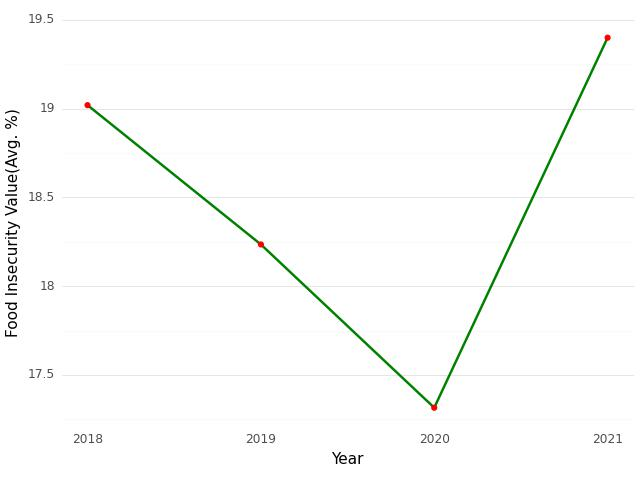
\includegraphics[width=0.75\linewidth]{images/food_insecurity_canada.jpeg}
\caption{\label{fig:food_insecurity_canada} Food-Insecurity Status in Canada}
\end{figure}

In Canada, average percentage of food insecurity was in the range from 17-19.5\% approximately. The value was around 19\% in 2018, which gradually decreased more or less 0.7\% in 2019. The best scenario is seen in 2020 when the percentage reached to a fall of 17.2\%. However, the trend drastically showed a 2\% increase over a year(2021).

Towards provinces, an interesting pattern is observed for Quebec which has the lowest percentage of food insecurity than all other provinces in Canada. Furthermore, most of the provinces had downward trend till 2019, then a sharp rise was seen for states:  Ontario(20\%), Manitoba(22\%), Saskatchewan(22.5\%), Nova Scotia(23\%) and Prince Edward Island(25\%, highest). In the meantime of Pandemic(2020), the figure shows a slight upward pattern, though New Brunswick and Alberta hit a increase by 4\% and 2\% respectively. In 2021, there was a dramatic rise in the number of people facing food insecurity in all the provinces except Saskatchewan. On the contrary, Newfoundland and Labrador reached the peak value at around 26\% which is the highest in this figure.

\begin{figure}
\centering
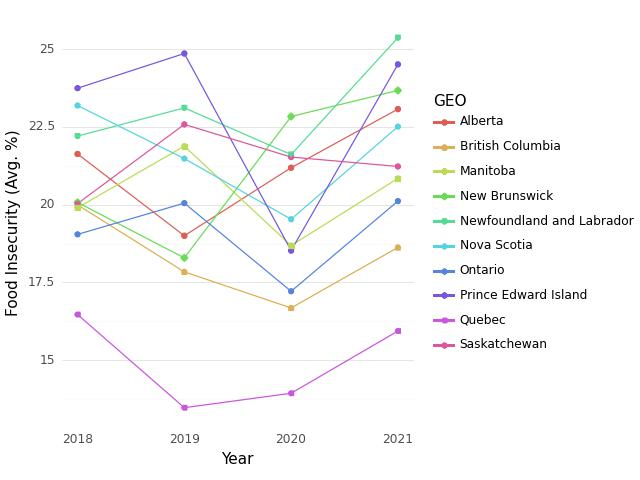
\includegraphics[width=0.75\linewidth]{images/food_insecurity_provinces.jpeg}
\caption{\label{fig:food_insecurity_provinces} Food-Insecurity Status across Provinces}
\end{figure}

For better understanding, four categories of household food insecurity status are analyzed along with provinces which are food security, insecurity, severe food insecurity, and moderate food insecurity and this illustration is presented on \href{https://sujana27.shinyapps.io/cse780-assignment-one}{Shiny app} \cite{shinyapp}.

\section{Conclusion}
Despite being a highly developed country, food insecurity is rapidly increasing in all over the provinces/territories in Canada. Although the trend fluctuates over the 4-year period, the gist data represents a increase pattern lately across all the provinces in Canada. This analysis plays a vital role to meet one the most valuable sustainable development goal in Canada which is ``End hunger, achieve food security''. 

\newpage
\section{Technical Supplemental Materials}
\begin{verbatim}
# Imports
import plotnine as plt9
from plotnine import ggplot, geom_point, aes, stat_smooth, facet_wrap
# Read the data
df_00 = pd.read_csv("dataset/13100834.csv")

# Filter out empty data and pre process the data
df_0 = df_00.drop(columns=['SYMBOL', 'TERMINATED'])
df_1 = df_0.loc[df_00['Statistics'] == "Percentage of persons"]
df_2 = df_1.loc[df_00['Household food security status'] == "Food insecure"]
df_3 = df_2.dropna(subset=['VALUE'])
cl_df = df_3[['GEO', 'REF_DATE','Household food security status', 'VALUE' ]]
cl_CA_df = cl_df.loc[cl_df['GEO'] == "Canada"]
cl_CA_df_2 = cl_CA_df.groupby(cl_CA_df['REF_DATE'])["VALUE"].mean()
years = cl_CA_df['REF_DATE'].unique()
np_arrray = np.asarray(cl_CA_df_2)
df_CA = pd.DataFrame(years, np_arrray)

## Plot Figure 1: Food Insecurity Status in Canada
plot = (
      plt9.ggplot(df_CA, mapping = plt9.aes(x = years, y=np_arrray)) +
      plt9.theme_minimal() +
      plt9.geom_line(linetype = "solid", size=1, color='green')+
      plt9.geom_point(color='red')+
      plt9.labs(x = "Year", y = "Avg. percentage of Food Insecurity Value", title="Figure 1: Food Insecurity Status in Canada") +
      plt9.theme(panel_grid_major_x = plt9.element_blank(), panel_grid_minor_x = plt9.element_blank())
  )
plot.draw()


ref_dates = cl_df['REF_DATE'].unique()
geos = ["Nova Scotia", "New Brunswick", "Quebec", "Ontario", "Manitoba", 
        "Saskatchewan", "Alberta", "Newfoundland and Labrador", 
        "Prince Edward Island", "British Columbia"]
my_array = []
for ref_date in ref_dates:
    for geo in geos:
        cl_NSc_df = cl_df[(cl_df.GEO == geo) & (cl_df.REF_DATE== ref_date)]
        mean_rslt = cl_NSc_df["VALUE"].mean()
        my_array.append([geo, ref_date, mean_rslt])
df = pd.DataFrame(my_array, columns = ['GEO','REF_DATE','VALUE'])


#Plot Figure 2:  Food-Security Status across Provinces

plot = (
      plt9.ggplot(df, mapping = plt9.aes(x = 'REF_DATE', y='VALUE', 
      color='GEO', group=df['GEO'])) +
      plt9.theme_minimal() +
      plt9.geom_line(linetype = "solid")+
      plt9.geom_point()+
      plt9.labs(x = "Year", y = "Avg. percentage of Food Secure Status") +
      plt9.geom_point(aes(shape=df['GEO'])) +
      plt9.theme(panel_grid_major_x = plt9.element_blank(), 
      panel_grid_minor_x = plt9.element_blank())
  )
plot.draw()
\end{verbatim}

\newpage
\section{Technical Supplemental Materials for Shiny}
\begin{verbatim}
import plotnine as plt9
from plotnine import aes
import pandas as pd
import numpy as np
from shiny import *

# read in data
df = pd.read_csv("13100834.csv")

# Function for UI
def create_ui():
  # create our ui object
  app_ui = ui.page_fluid(
    
    # App title ----
    ui.panel_title("Food Security Status in Canada"),
    
    # Subtitle
    ui.markdown(
        """
        Dataset: [Food insecurity by economic family type]
        (https://open.canada.ca/data/en/dataset/a98ab5ae-c484-41d0-815c-b71562ed0704)
        """
    ),
    ui.row(
        # line chart output
        ui.column(10, ui.output_plot("barplot")), 
        # controls
        ui.column(2,
           
          ui.markdown(
            """
            **Select food secure status and province to explore**
            """
          ),
          ui.input_select(
              "secure_status", "Food Secure Status",
              choices=["Food insecure", "Food secure", "Food insecure, severe", "Food insecure, marginal"],
              selected=["Food insecure"]
          ),
          ui.input_checkbox_group(
              "geo_locations", "Locations",
              choices=["Nova Scotia", "New Brunswick", "Quebec", "Ontario", 
              "Manitoba", "Saskatchewan", "Alberta", "Newfoundland and Labrador", 
              "Prince Edward Island", "British Columbia"],
              selected=["Nova Scotia", "New Brunswick", "Quebec", "Ontario", 
              "Manitoba", "Saskatchewan", "Alberta", "Newfoundland and Labrador", 
              "Prince Edward Island", "British Columbia"]
          )
        ),
    )
  )
  return app_ui

ui_obj = create_ui()


# Function to make the plot
def create_plot(data):
  plot = (
    plt9.ggplot(data = data, mapping = plt9.aes(x = 'REF_DATE', y='VALUE', 
                color='GEO', group=data['GEO'])) +
      plt9.theme_minimal() +
      plt9.geom_line(linetype = "solid")+
      plt9.geom_point()+
      plt9.labs(x = "Year", y = "Avg. Food Status(%)", title="Food-Security Status over the years") +
      plt9.geom_point(aes(shape=data['GEO']))+
      plt9.theme(panel_grid_major_x = plt9.element_blank(), panel_grid_minor_x = plt9.element_blank())
  )
  return plot.draw()


def generate_mean_of_data(cl_df):
  ref_dates = cl_df['REF_DATE'].unique()
  geos = cl_df['GEO'].unique()
  my_array = []
  for ref_date in ref_dates:
    for geo in geos:
      cl_NSc_df = cl_df[(cl_df.GEO == geo) & (cl_df.REF_DATE== ref_date)]
      mean_rslt = cl_NSc_df["VALUE"].mean()
      my_array.append([geo, ref_date, mean_rslt])

  df = pd.DataFrame(my_array, columns = ['GEO','REF_DATE','VALUE'])
  return df 


# Function for the server
def create_server(data):
  
  def f(input, output, session):
    @output(id = "barplot")
    @render.plot
    def plot():
      req(input.geo_locations())
      req(input.secure_status())

      geo_location = list(input.geo_locations())
      food_secure_status = input.secure_status()
      food_sec_data = data.loc[data['Household food security status'] == food_secure_status]
      mean_data = generate_mean_of_data(food_sec_data)
      plot_data = mean_data[mean_data['GEO'].isin(geo_location)]
      plot = create_plot(plot_data)
      return plot
  return f

# Filter out empty data and pre process the data
df_0 = df.drop(columns=['SYMBOL', 'TERMINATED'])
df_1 = df_0.loc[df['Statistics'] == "Percentage of persons"]
#df_2 = df_1.loc[df['Household food security status'] == "Food insecure"]
df = df_1.dropna(subset=['VALUE'])
cl_df = df[['GEO', 'REF_DATE','Household food security status',  'VALUE' ]]

server = create_server(cl_df)
app = App(ui_obj, server)

\end{verbatim}

\newpage
\bibliographystyle{IEEEtran}
% Loading bibliography database
%\bibliography{reference}
\bibliography{sample}

\end{document}